%
% Space-Based Quantum Networks
%

\section{Space-based quantum networks}\label{sec:quant_space_race}\index{Space race}\index{Satellites}

\dropcap{O}{ne} of the major hurdles that must be overcome before quantum networks achieve widespread commercial use is to span large distances between nodes distributing entanglement as a resource. The key technological and commercial centres of the world are decentralised, spread across the globe, hence connections over intercontinental distances are essential, with nodes separated potentially by thousands of kilometres. This distance is one of the major challenges facing the creation of large-scale quantum networks.

The most convenient way of transmitting quantum information is using optical fibres\index{Optical fibres}. However, it is well-known that due to the exponential scaling of loss with distance, the upper limit is of the order of several hundred kilometres. This shortcoming has inspired intensive research into extending these distances using quantum repeaters, discussed in detail in Sec.~\ref{sec:rep_net}\index{Quantum repeater networks}.

An alternative to fibre optic communication is using terrestrial free-space links\index{Terrestrial free-space communication}. Particular wavelength regimes exhibit low absorption\index{Absorption}, allowing the propagation of photons across long distances. Impressive experimental demonstrations of teleportation with free-space entanglement \cite{bib:NP_3_481, bib:Nat_489_269, bib:yin2013lower} over 100km have been achieved.

However, extending to longer distances has been problematic. Photon loss in free-space links is affected by weather\index{Weather conditions} conditions and other atmospheric effects\index{Atmospheric effects}\index{Photon loss}, such as pollution\index{Pollution}, which degrade visibility. The Earth's curvature\index{Earth curvature} provides an absolute upper limit, depending on the elevation of the source and receiver. For example, for an observer on a 30m tower, the horizon is at a distance of 20km, a relatively short distance. The observatory used in the experiments performed by the experiments of \cite{bib:NP_3_481, bib:Nat_489_269} were at an elevation of 2393m, allowing transmission over a distance of 143km.

In general, the distance to the horizon $d$ (in kilometres)\index{Distance to horizon} on the Earth's surface at an altitude of $h$\index{Ground station altitude} (in metres) is given by the approximation,
\begin{align}
d \approx 3.57\sqrt{h}.
\end{align}
This relationship is shown in Fig.~\ref{fig:dist_hor}, covering the range of altitudes from sea level\index{Sea level} to the summit of Mount Everest (8,848m)\index{Mount Everest}. It is evident that line-of-sight\index{Line-of-sight} channels across the Earth's surface are inherently limited by the curvature of the Earth to $\sim$250km, using altitudes that are practically realistic (i.e no ground stations on the summit of Everest thank you very much!).

\begin{figure}[!htbp]
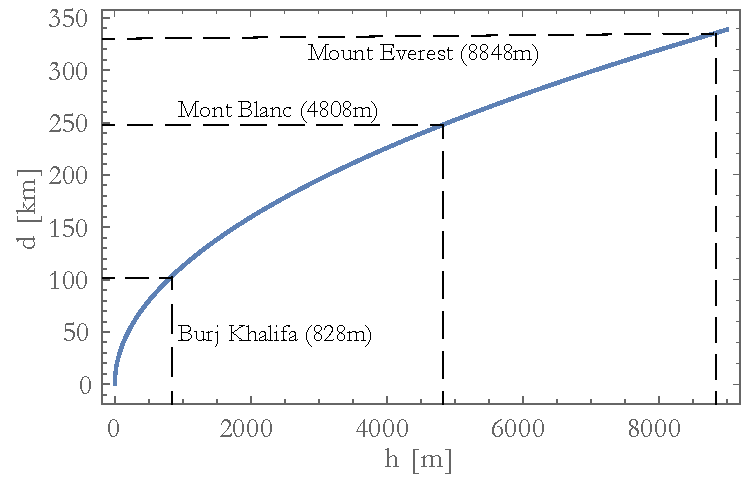
\includegraphics[clip=true, width=0.475\textwidth]{distance_to_horizon}
\captionspacefig \caption{Distance to the horizon $d$ (in kilometres), at altitude $h$ (in meters), and several illustrative examples with their elevations. The range for $h$ spans from sea level to roughly the height of Mount Everest, thereby covering the full range of altitudes possible for ground-based network nodes. However, using more practically realistic bounds on altitude, say on the order of 5,000-6,000m (already very optimistic, and only achievable in some parts of the globe), line-of-sight distance to the horizon will be limited to be on the order of 200-250km. This limitation necessitates the use of repeater networks to enable the efficient approaches for constructing quantum communication channels that bypass this constraint imposed by the Earth's curvature.\index{Mount Everest}\index{Mont Blanc}\index{Burj Khalifa}} \label{fig:dist_hor}
\end{figure}

One attractive possibility to overcome these issues is using space-based quantum communication. In this scenario, satellites orbiting the Earth would act as nodes of the quantum network, which could store, send and receive quantum information. At altitudes where satellites orbit the Earth, photon loss due to scattering\index{Photon loss}\index{Scattering} is negligible, and photons can propagate across extremely long distances unhindered -- despite various shortcomings of photonic quantum information, a key benefit is their robustness and preservation of coherence through empty space over very long distances. The main loss in this case is caused by diffraction\index{Diffraction}, due to the finite diameter of the receiver and transmitter hardware. For example, using reasonable diameters it is in the region of 40-80dB loss for low Earth orbit (LEO)\index{Low Earth orbit} satellites \cite{bib:aspelmeyer2003long, bib:liao2016ground}.

Repeater network protocols (Sec.~\ref{sec:rep_net}) are completely compatible in-principle with the space-based networks discussed here. In the context of a space-based network the key limitation we face is that the opposing hemisphere of the Earth is beyond direct line-of-sight\index{Line-of-sight}, prohibiting a direct P2P\index{Point-to-point} communications channel. Instead, the long-distance channel must be broken down into shorter segments, within line-of-sight of one another, enabling, for example, entanglement to be incrementally swapped\index{Entanglement swapping} across neighbouring satellites and ultimately around the globe.

Involving ground-based quantum network nodes is not an inherent problem as 80\% of the atmosphere by mass is located within the first 12km in altitude, yielding low effective thickness of the atmosphere ($\sim10$km)\index{Effective atmospheric thickness}. This effective thickness of course changes with the azimuth of the satellite in the sky. Near the horizon the line-of-sight\index{Line-of-sight} between satellite and ground-station is far greater than when the satellite is directly overhead. The light trajectory beyond this effective thickness regime effectively passes through vacuum with attenuation\index{Photon loss} limited only by diffraction\index{Diffraction}. Thus, when directly overhead, a satellite-to-ground\index{Satellite-to-ground communication} channel is more favourable in terms of signal attenuation than long-distance ground-to-ground\index{Ground-to-ground communication} channels.

Ground-to-satellite\index{Ground-to-satellite communication} and satellite-to-ground\index{Satellite-to-ground communication} quantum communication have already been demonstrated, as will be discussed in detail in the next section. Such a satellite-based quantum communication system is naturally suited to various tasks, in particular QKD\index{Quantum key distribution (QKD)}, which does not require quantum memories\index{Quantum memory} or impose onerous timing constraints. However, with the addition of quantum memories the capabilities of such a quantum network could be greatly enhanced, enabling many of the applications and protocols described earlier (Part.~\ref{part:protocols}) at a global scale.

Naturally, such a space-based quantum network brings with it enormous engineering challenges that must be overcome prior to implementation. Creating even a short-distance quantum network is currently technologically challenging, let alone one that is loaded onto a satellite transmitting photons across distances potentially of the order of the diameter of the Earth. The cooperation of space agencies is necessary even for initial experiments.

As we describe more in the next section, several recent positive results have made the technology an immediate possibility in realising such a global level quantum network. In this section, we summarise the current technological state of the art internationally, and discuss some of the remaining major challenges.  

There are two main ingredients for communication in a global satellite-based quantum internet: satellite-to-satellite\index{Satellite-to-satellite communication}, and ground-to-satellite\index{Ground-to-satellite communication}, shown in Fig.~\ref{fig:space_1}. Each bring with them their own engineering challenges.

\if 2\pubmode
\begin{figure}[!htbp]
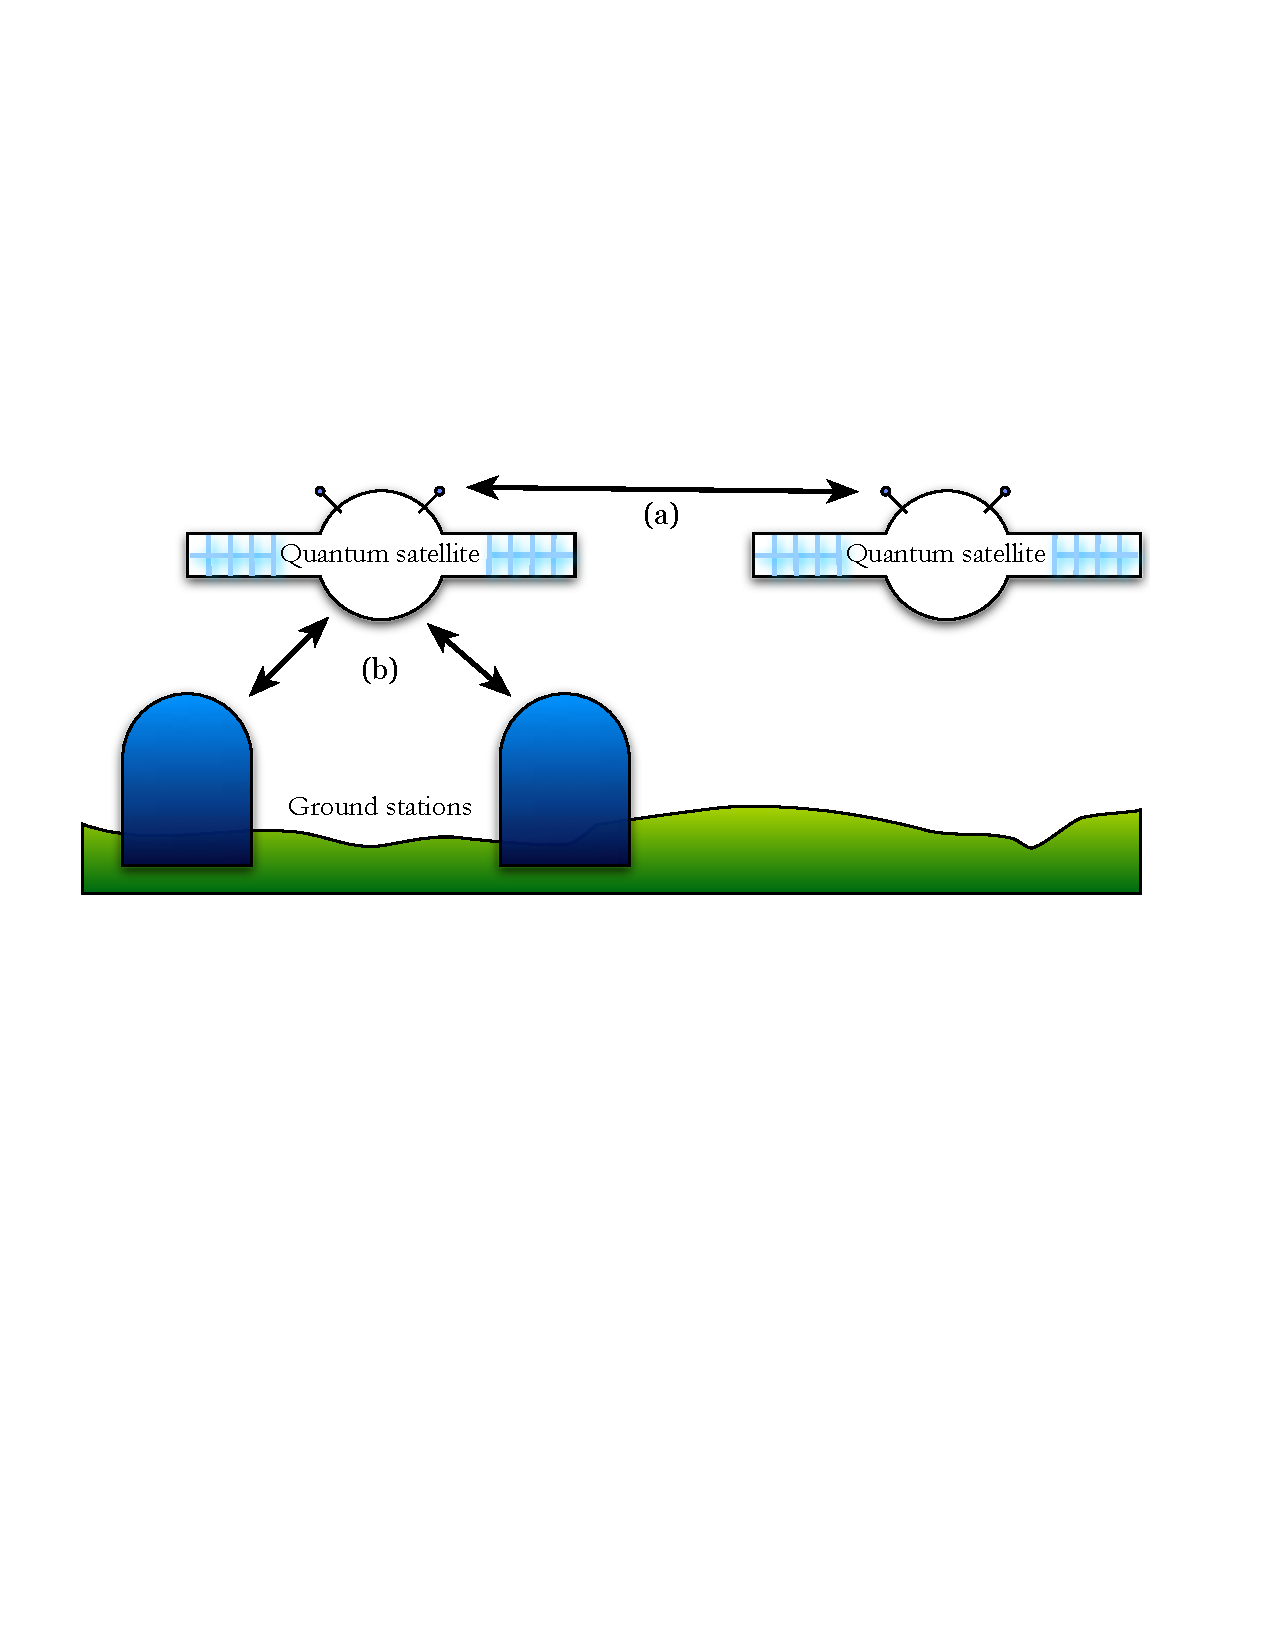
\includegraphics[clip=true, width=0.475\textwidth]{satellite_configs}
\captionspacefig \caption{\comment{Bigger in 1 column}Various possibilities for space-based quantum communication. (a) Satellite-to-satellite quantum communication \cite{bib:byrnes2017lorentz}. (b) Ground-to-satellite quantum communication \cite{bib:armengol08}.}
\label{fig:space_1}
\end{figure}
\else
\begin{figure*}[!htbp]
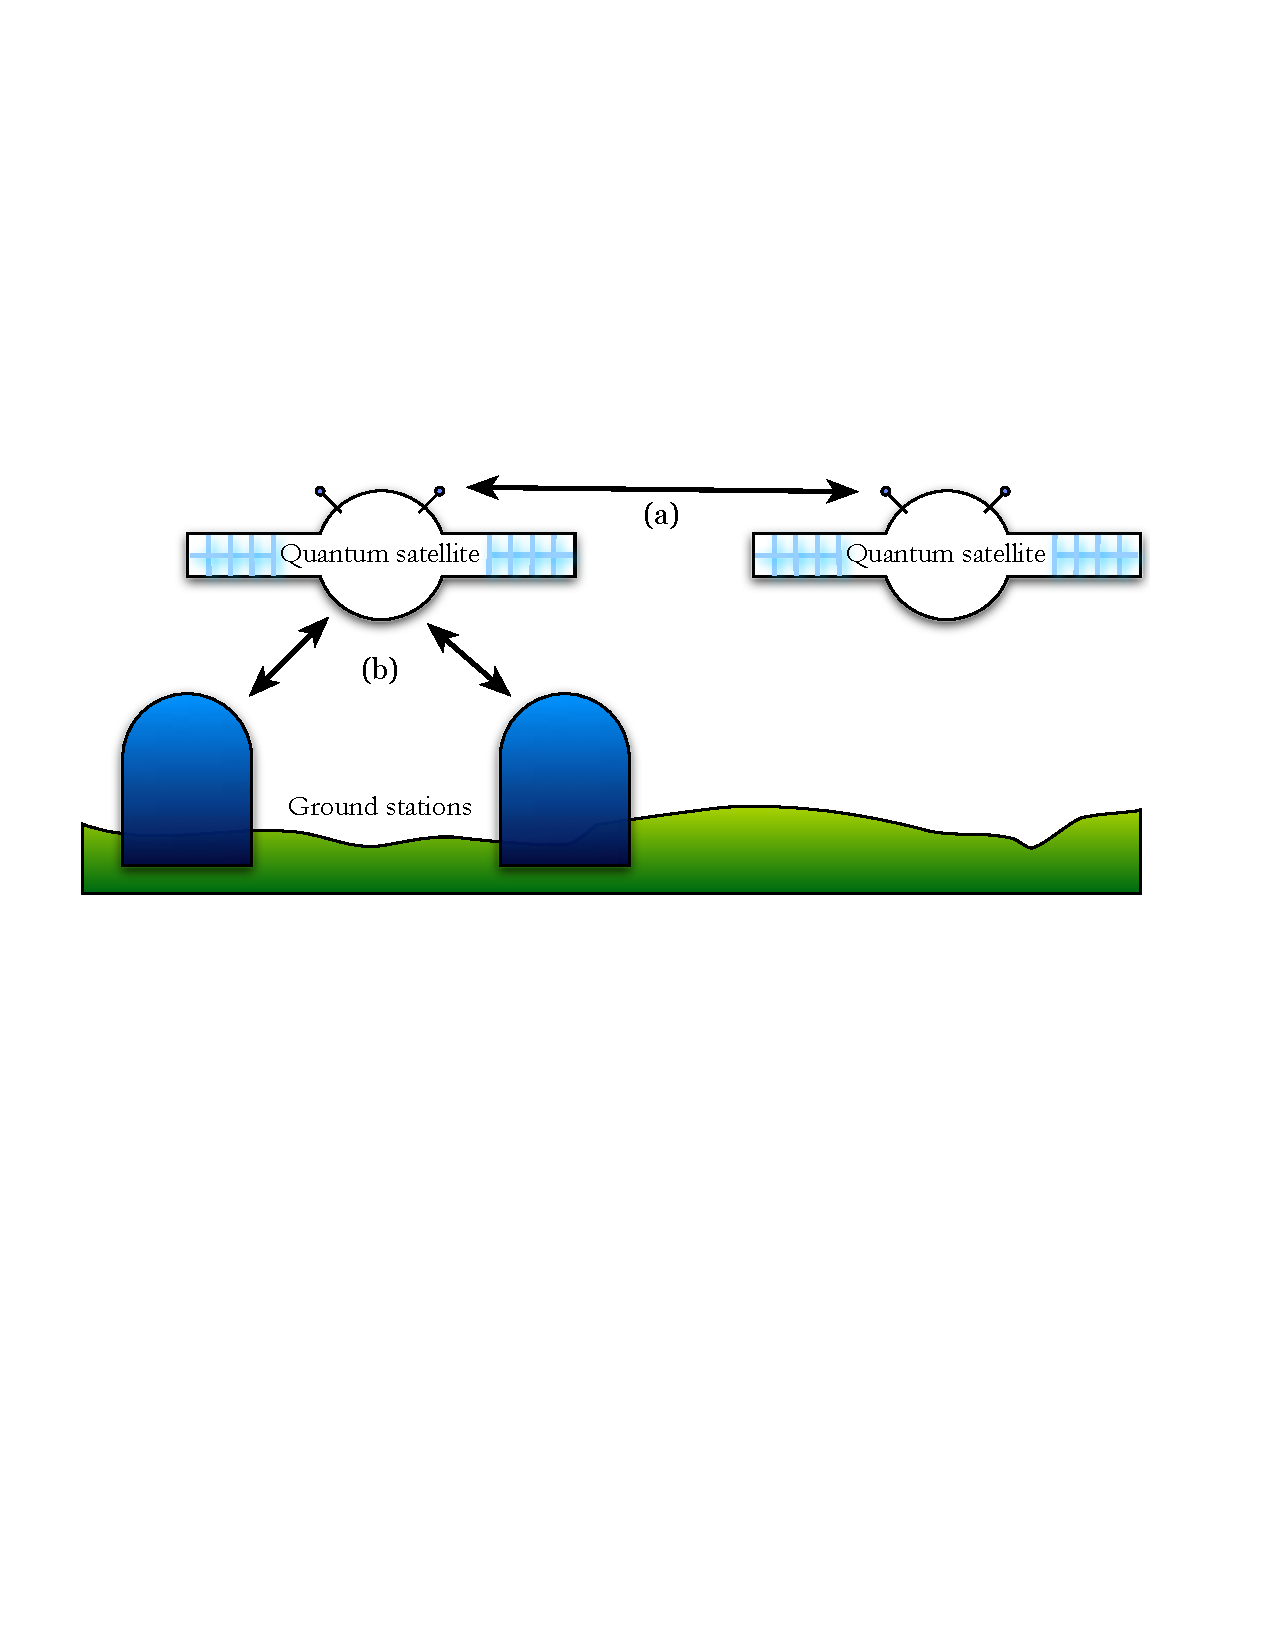
\includegraphics[clip=true, width=\textwidth]{satellite_configs}
\captionspacefig \caption{Various possibilities for space-based quantum communication. (a) Satellite-to-satellite quantum communication \cite{bib:byrnes2017lorentz}. (b) Ground-to-satellite quantum communication \cite{bib:armengol08}.}
\label{fig:space_1}
\end{figure*}
\fi 

%
% International efforts for space-based quantum communication
%

\subsection{International efforts}\index{International efforts}

We now briefly summarise some of the major international developments in the demonstration of satellite-based quantum communication. Some of these developments are extremely recent at the time of writing this work. It is a certainty that major developments will follow in the near future, with increasingly capable satellites, enabling the demonstration of ever more sophisticated quantum protocols.

\begin{figure*}[!htbp]
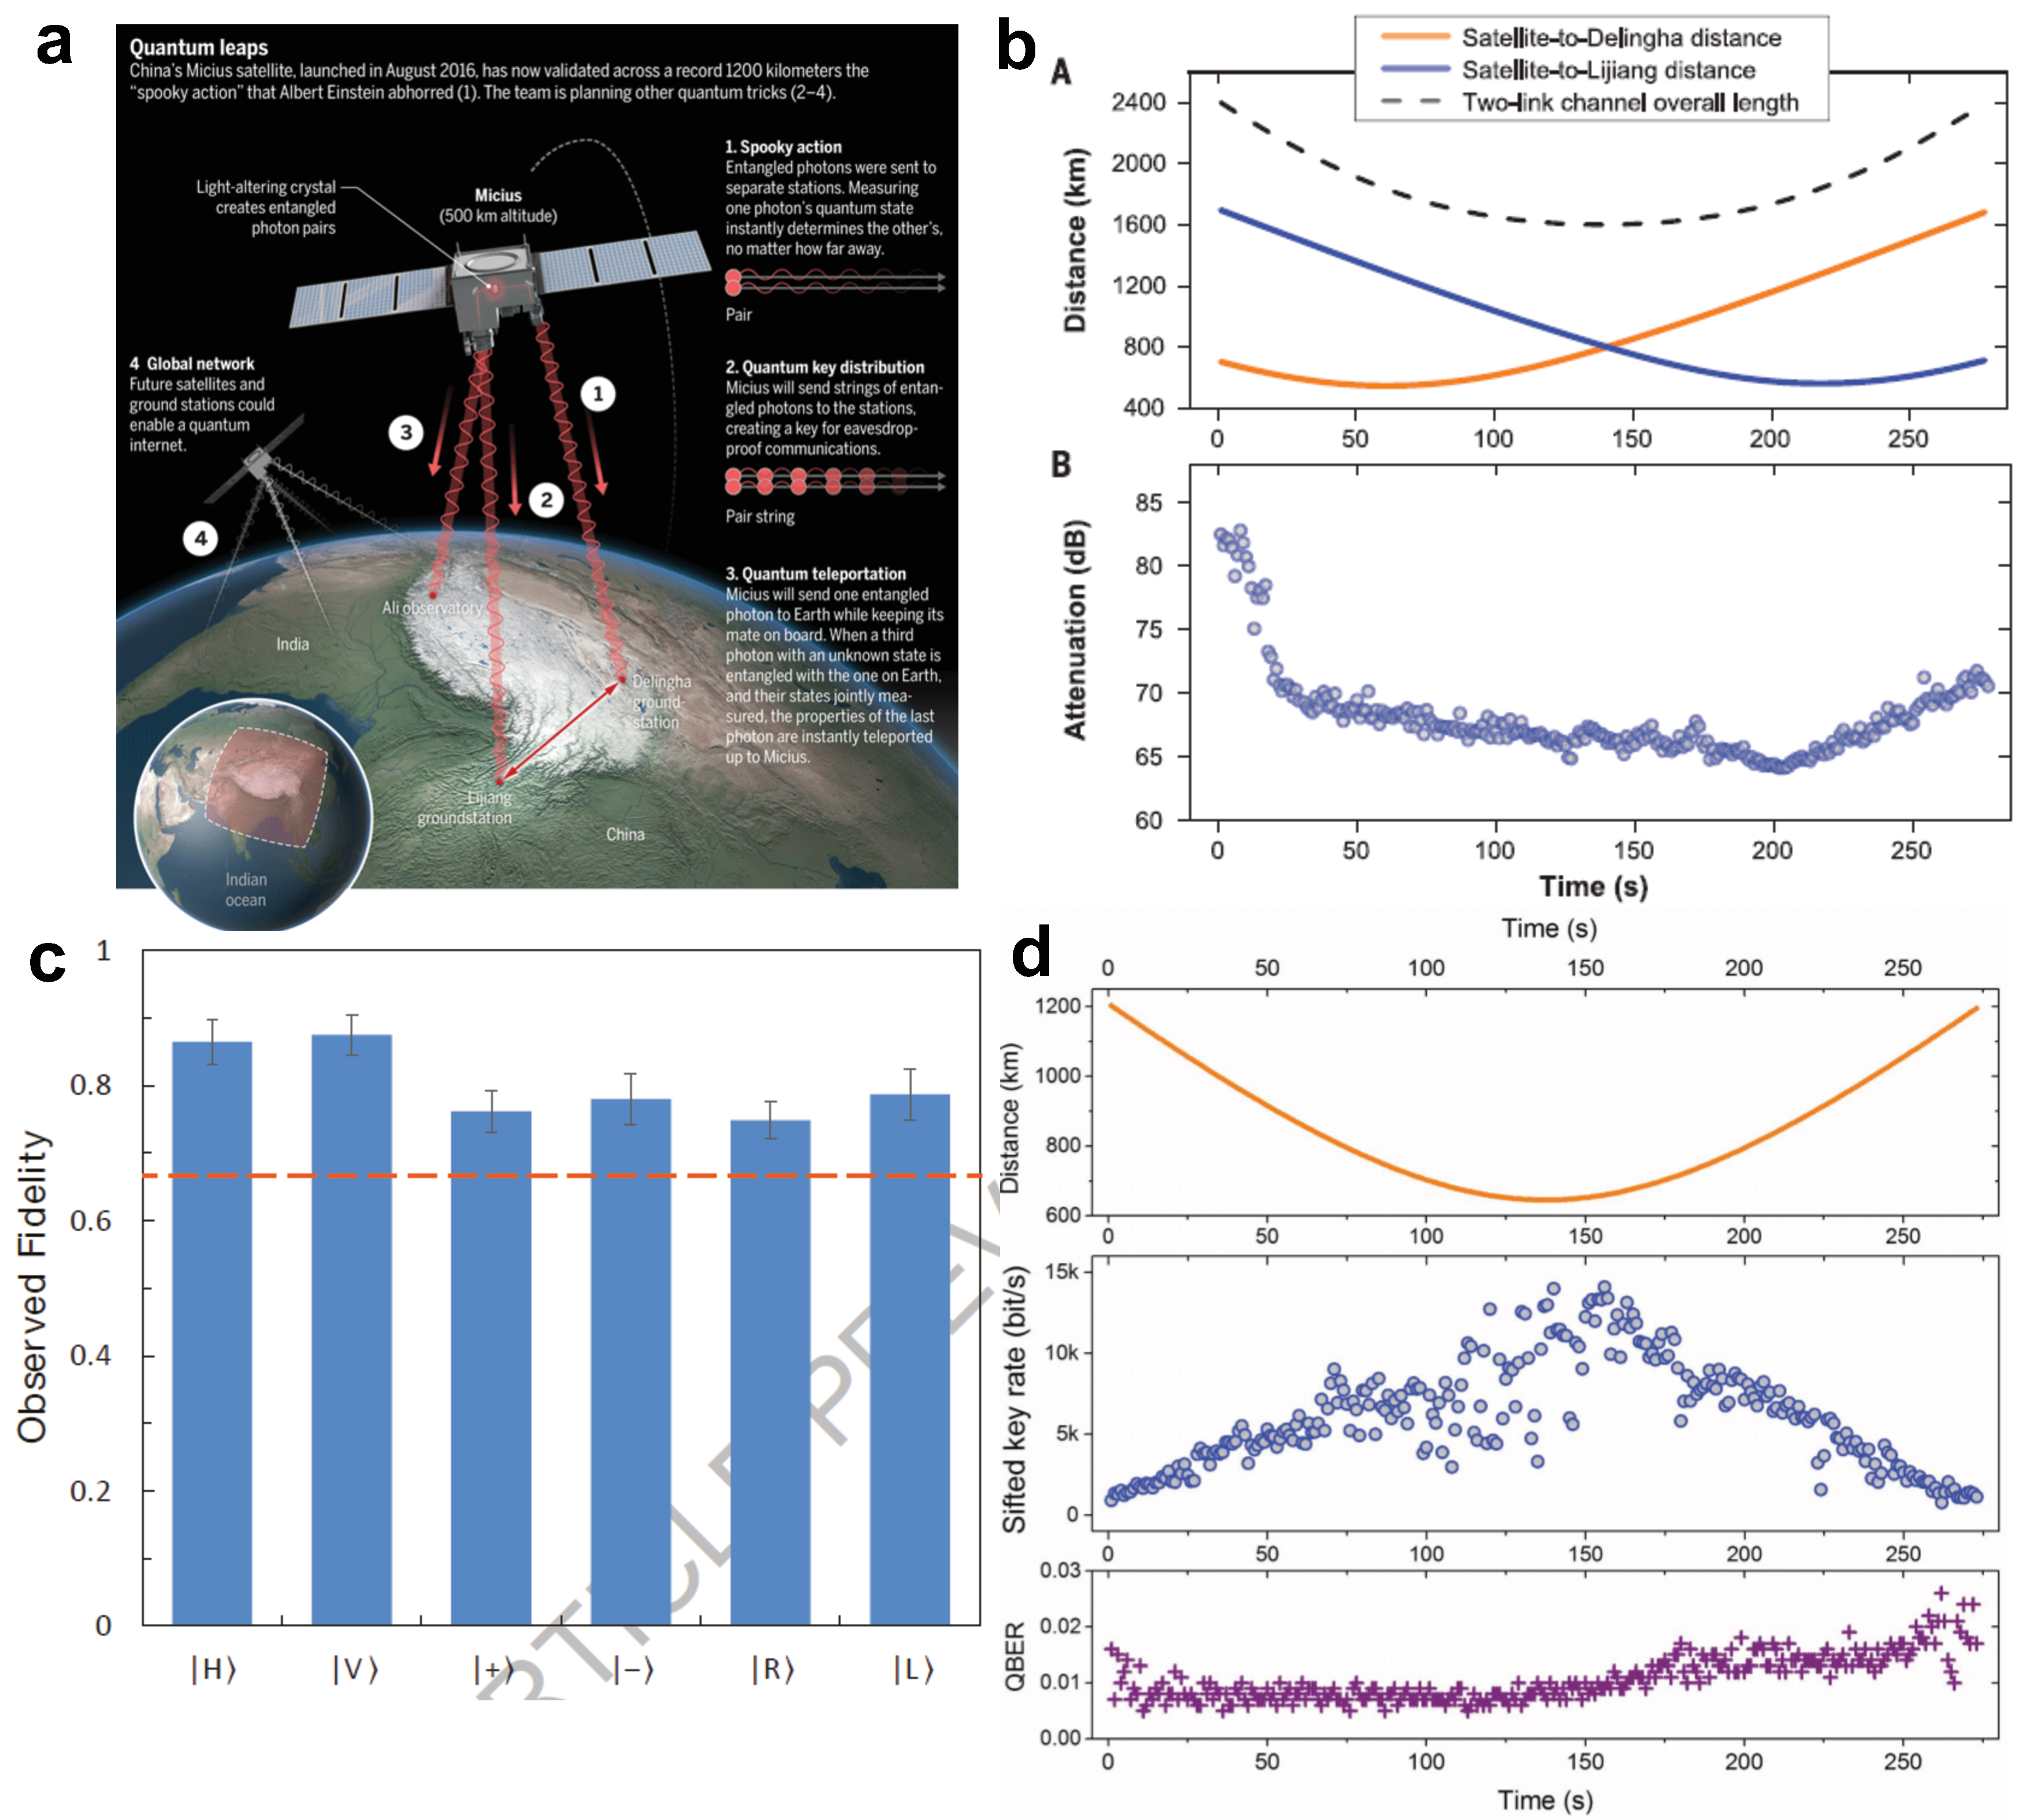
\includegraphics[clip=true, width=\textwidth]{space_4}
\captionspacefig \caption{The Chinese Micius quantum communications satellite. (a) Schematic of the satellite and ground stations used to observe the entangled photons \cite{bib:popkin17}. \comment{[TB: Took image from Science News, may need permission]. Picture is watermarked}. (b) Attenuation during entanglement distribution from \cite{bib:yin2017satellite}. (c) Fidelities achieved for teleportation of various states as marked from \cite{bib:ren2017ground}.}
\label{fig:space_4}
\end{figure*}

%
% China: QUESS
%

\subsubsection{China: QUESS}\index{QUESS}

In 2016, the group at the University of Science \& Technology China (USTC), led by Jian-Wei Pan\index{Jian-Wei Pan}, launched QUESS (Quantum Science Experiment Satellite), a quantum communication satellite \cite{bib:N_535_478, bib:xin11}. The main feature of the satellite is an ultra-bright source of polarisation entangled photons at a wavelength of 810nm, generated by SPDC\index{Spontaneous parametric down-conversion (SPDC)}. The source is capable of emitting $5.9 \times 10^6$ photon-pairs per second with a fidelity of $\sim 0.91$.

The other important piece of technology is the acquisition, pointing, and tracking technology\index{Acquisition}\index{Pointing}\index{Tracking}, which allows the ground stations to track the location of the satellite as it moves across the sky (which is very rapid for LEO), and vice versa. This is achieved using lasers at separate wavelengths, and allows the photon transmission and the ground-based receivers to be pointing to each other to within $\sim 1.2$mrad \cite{bib:yin2017satellite}. The major aims of the project are to: perform QKD\index{Quantum key distribution (QKD)} between Xinglong and Urumqi (a ground distance of 2,500km); test Bell's inequality\index{Bell inequality} across a distance of 1,200km; and perform QST\index{Quantum state teleportation} between the satellite and Ali in Tibet (see Fig.~\ref{fig:space_4}). The final aim is to perform QKD between Beijing and Vienna (a distance of 7,500km that extends well beyond the Earth's curvature). 

At the time of writing, three main results have been reported. The first is an entanglement distribution experiment where a Bell violation was observed between ground stations at Delingha and Lijiang (separated by 1,203km) and Delingha and Urumqi (separated by 1,120km) \cite{bib:yin2017satellite}. The satellite is in LEO at an elevation of $\sim500$km, and is in view from the observatories for a narrow duration of $\sim275$s.

The attenuation of the photons during the downlink transmission is shown in Fig.~\ref{fig:space_4}(b). Taking into account photon transmission distances, the attenuation rates are far better than the best performance of optical fibres at 0.16dB/km \cite{bib:yin2013lower} and even theoretical loss limits. The Bell violation recorded in this experiment was at the level of $2.37\pm 0.09>2$, and the non-locality\index{Non-locality} of the entanglement was confirmed.

The second experiment performed ground-to-satellite\index{Ground-to-satellite communication} QST\index{Quantum state teleportation} \cite{bib:ren2017ground}. Here a single polarisation-encoded photon defines the qubit to be teleported, and the satellite acts as the receiver. The entangled photons are generated on the ground, at the observatory in Ngari, Tibet. As with the first experiment described above, the satellite is in LEO and sweeps across the sky, creating a narrow time-window during which the teleportation must be achieved. The longest distance for successful teleportation was $\sim 1400$km, when the satellite emerges from the horizon. When directly overhead, the satellite is at a distance of $\sim 500$km. As Fig.~\ref{fig:space_4}(c) shows, the fidelity of the types of states teleported are all above the theoretical classical bound of $2/3$, with an average of $0.80 \pm 0.01$.  

A third experiment performed QKD in a satellite-to-ground\index{Satellite-to-ground communication} configuration, where the ground station was at Xinglong \cite{bib:liao2017satellite}. The protocol that was used was the decoy-state BB84\index{Decoy-states}\index{BB84 protocol} protocol, which is robust against a photon-number splitting attack\index{Photon-number splitting attack}. A key-rate of between $1-12$kbit/s was achieved while the satellite was visible, depending upon the relative location in the sky, shown in Fig.~\ref{fig:space_4}(d).

%
% Japan: SOCRATES
%

\subsubsection{Japan: SOCRATES}\index{Space Optical Communications Research Advanced Technology Satellite (SOCRATES)}

SOCRATES (Space Optical Communications Research Advanced Technology Satellite) is a micro-satellite\index{Micro-satellites} developed by NICT (National Institute of Information \& Communications Technology\index{National Institute of Information \& Communications Technology (NICT)}) \cite{bib:horiuchi2015view, bib:toyoshima2015current, bib:takenaka2017}. This is a 48kg satellite of volume $50^3$cm$^3$ that demonstrates multi-purpose (i.e. both classical and quantum) optical communication. Its primary mission is to demonstrate laser communication in space. As one of its subgoals, the on-board equipment is adapted to perform QKD experiments\index{Quantum key distribution (QKD)}. To this end, the satellite is equipped with a photon source, where the polarisation can be classically switched between non-orthogonal angles, necessary for BB84\index{BB84 protocol} for example.

Initial results indicated polarisation preservation of photons emitted from the satellite, a preliminary step towards performing protocols such as BB84\index{BB84 protocol} \cite{bib:carrasco2016leo}. More recent results showed quantum-limited satellite-to-ground\index{Satellite-to-ground communication} communication was possible, attaining a quantum bit error rate below 5\% \cite{bib:takenaka2017} during the closest approach of the satellite to the ground at a distance of 744km. The downlink was established over distances of over 1,000km, although for obvious reasons the error rate was higher for longer distances.

%
% Singapore: Cubesat
%

\subsubsection{Singapore: Cubesat}\index{Cubesat}

The group at the National University of Singapore (NUS)\index{National University of Singapore (NUS)} also has taken the approach of using nano-satellites\index{Nano-satellites}, with the capability of generating correlated photon-pairs on-board \cite{bib:tang2016generation}. The nano-satellite weighs just 1.65kg and has all the components required for creating and detecting SPDC photon pairs. The nano-satellite approach greatly reduces the cost of space-launch, and the launch itself was performed by the Indian space agency \comment{What's it called}. As photon generation and detection are both on the same satellite, no quantum communications channel (to other satellites or Earth) was established in the experiment, although it demonstrated in-principle the space-worthiness of the basic hardware components. 

%
% Europe: Retroreflector Satellite
%

\subsubsection{Europe: Retroreflector satellite}\index{Retroreflector satellite}

European groups used laser-ranging satellites fitted with corner-cube\index{Corner-cube} retroreflectors\index{Retroreflector satellite} to demonstrate quantum communication through the atmosphere \cite{bib:NJP_10_033038, bib:vallone15}. A ground-based photon source transmitted photons towards the satellite, which reflected them back down again to an Earth-based observatory. This confirmed the ability of photons to travel through the atmosphere into space and back, with a bit error ratio at the level of 5\%. Although no optical sources or detectors were placed on the satellite, there has been long-standing active interest in a European space-based quantum communication project, led in particular by the group of Anton Zeilinger at the University of Vienna\index{University of Vienna} \cite{bib:armengol08}. The aims of such projects are to perform space-based QKD\index{Quantum key distribution (QKD)}, with terrestrial free-space experiments \cite{bib:NP_3_481, bib:Nat_489_269} a part of the overall research effort. 

%
% Canada: QEYSSat
%

\subsubsection{Canada: QEYSSat}\index{QEYSSat}

The QEYSSat (Quantum EncrYption \& Science Satellite) proposes a micro-satellite\index{Micro-satellites} that incorporates a quantum receiver \cite{bib:jennewein2014qeyssat}. The satellite acts as a trusted node\index{Trusted nodes}, to which photons would be transmitted from Earth-based sources. This could be employed to perform QKD between two locations on Earth separated by large distances. No photon sources or quantum memories would be included on the QEYSSat. 

\begin{figure*}[!htbp]
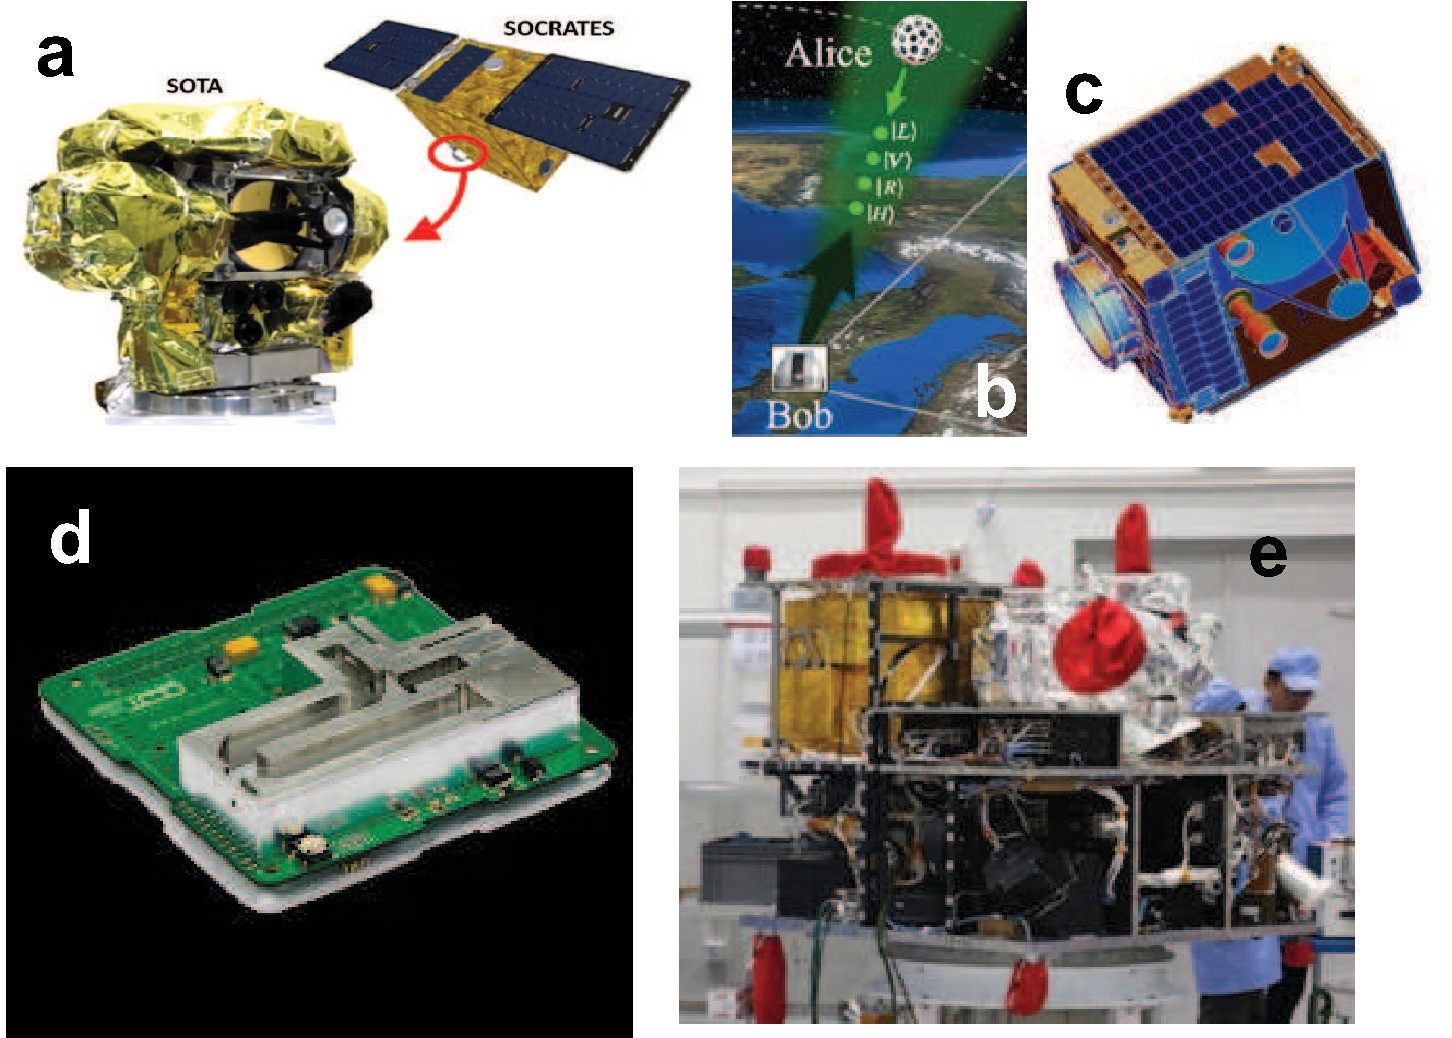
\includegraphics[clip=true, width=\textwidth]{space_2}
\captionspacefig \caption{Satellites employing quantum technologies from various groups across the world: Japan \cite{bib:horiuchi2015view}, Italy \cite{bib:vallone15}, Canada \cite{bib:jennewein2014qeyssat}, Singapore \cite{bib:tang2016generation}, and China \cite{bib:N_535_478}. \comment{Tim: do we have figure permission for this?}}
\label{fig:space_2}
\end{figure*}

%
% Future challenges
%

\subsection{Future challenges}

While early demonstrations of satellite-based quantum protocols have been successfully performed, future more sophisticated protocols will require more capable satellite hardware, which will inevitably begin to emerge in the immediate-term.

We identify two of the most pressing challenges facing a space-based quantum internet as:
\begin{itemize}
\item Coverage\index{Coverage}: how much of the surface of the globe will always be within line-of-sight of at least one satellite in the constellation network. Visibility of at least one satellite from any point on Earth will in-principle allow universal access to the quantum network, in the same way that the GPS constellation serves all points on the Earth's surface.
\item Precision\index{Precision}: many optical quantum protocols require strict synchronisation of photons undergoing interference. This becomes extremely challenging when those photons are originating from different satellite nodes, which must then be temporally synchronised on the scale of the photons' temporal wave-packets (i.e temporal mode-matching, discussed in Sec.~\ref{sec:MM_error}). Complicating things further, at satellite velocities relativistic effects become relevant to synchronisation. This is significant enough that the existing GPS\index{Global positioning system (GPS)} satellite positioning network must compensate for relativistic effects to maintain positioning accuracy.
\end{itemize}

%
% Coverage
%

\subsubsection{Coverage}\index{Coverage}

Currently there are only two satellites with the capability of sending and/or receiving photons through space: the Chinese QUESS\index{QUESS}, and the Japanese SOCRATES\index{Space Optical Communications Research Advanced Technology Satellite (SOCRATES)} satellites. In order to achieve world-wide coverage multiple communicating satellites will be necessary such that there be a constellation of satellites\index{Satellite constellation} that are visible at all times, anywhere on Earth, in a similar manner to the GPS satellite network\index{Global positioning system (GPS)}, thereby bypassing line-of-sight constraints, as per Fig.~\ref{fig:sat_constellation}.

\begin{figure}[!htbp]
	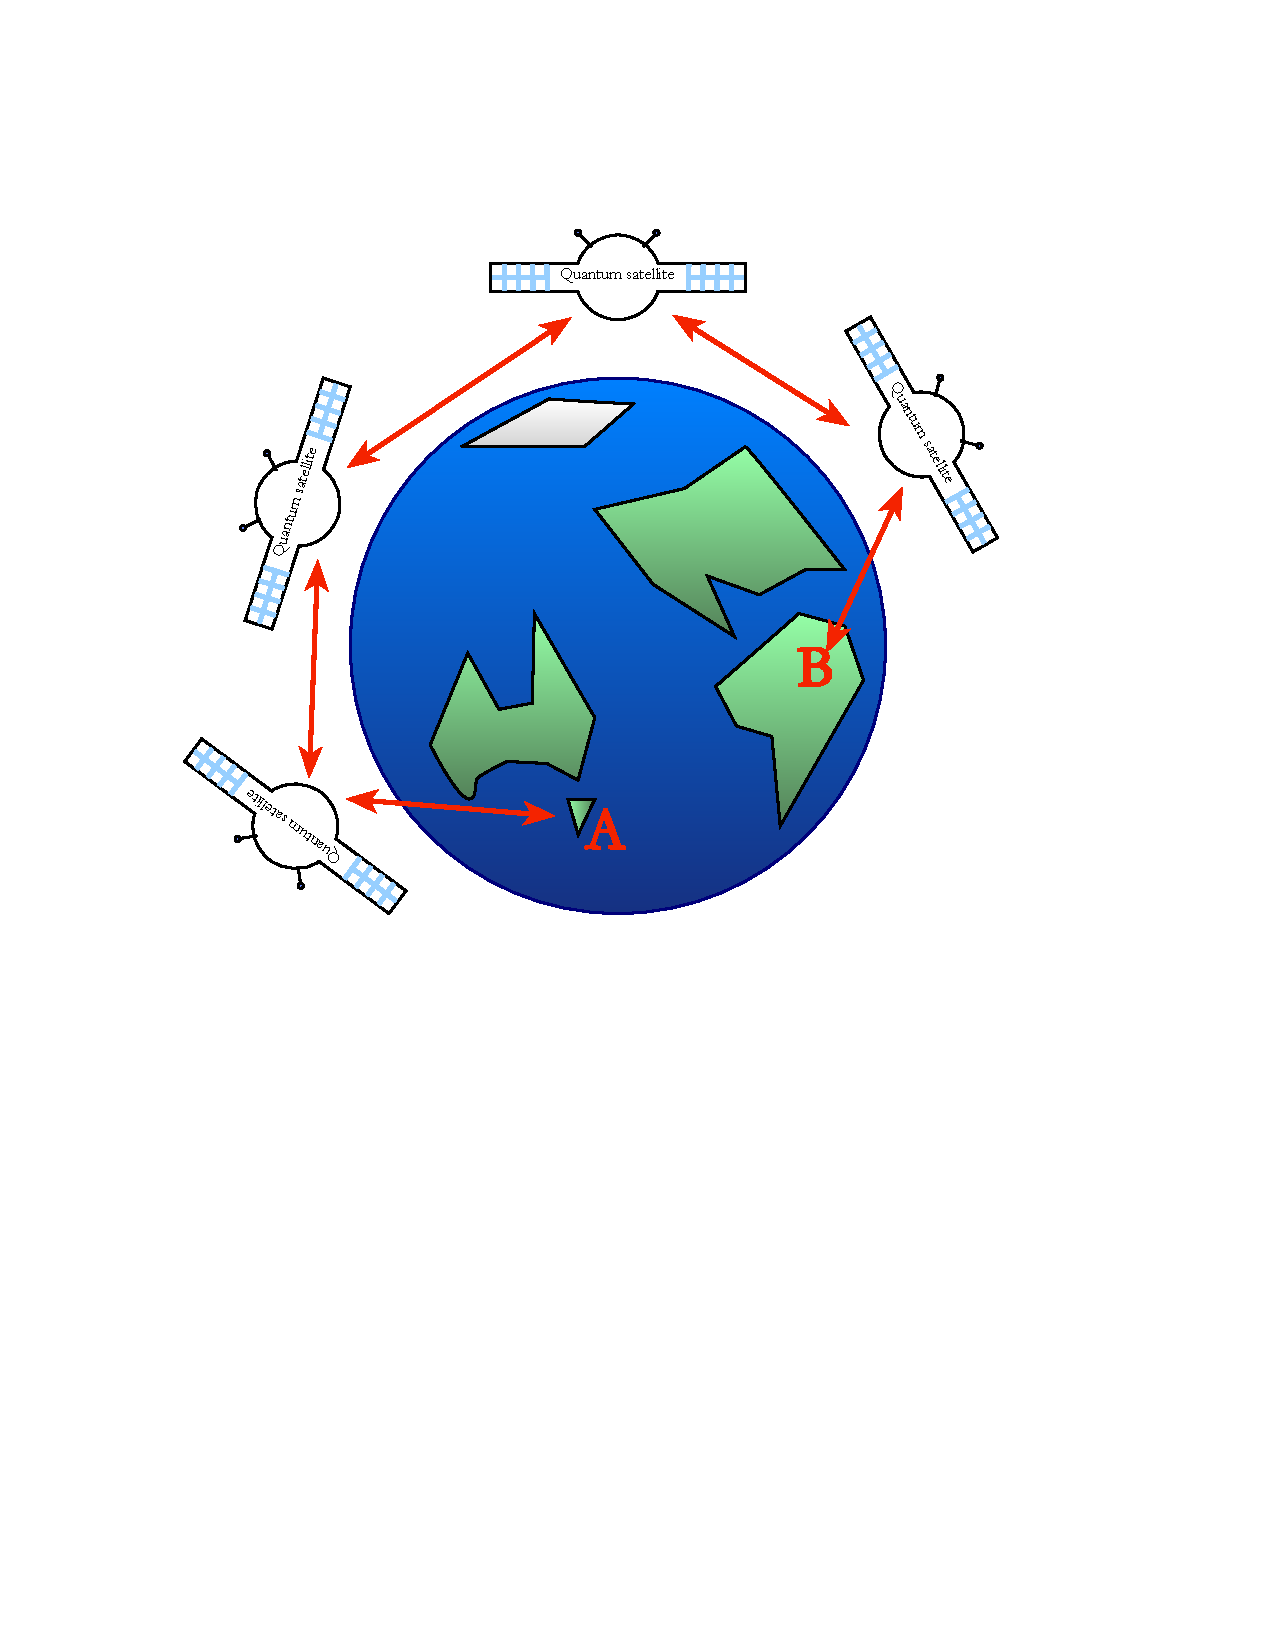
\includegraphics[clip=true, width=0.475\textwidth]{satellite_constellation}
	\captionspacefig \caption{Satellite constellation network for bypassing line-of-sight constraints in long-distance quantum communication. Neighbouring satellites connect via line-of-sight in space, and there are a sufficient number of satellites to enable global coverage such that all points on the Earth's surface are visible to at least one satellite at any given time, giving them indirect quantum access to any other point on the globe. In this simple example, entanglement swapping between satellites shares a Bell pair between Columbia and Tasmania, enabling the teleportation of certain Columbian products\index{Benzoylmethylecgonine} from Bogot{\'a} to the dance parties featuring at \href{https://soundcloud.com/peter-rohde}{DJ Rohde's} holiday home.\index{DJ Rohde}\index{Pablo Escobar}} \label{fig:sat_constellation}\index{Satellite constellation}
\end{figure}

In the case of the QUESS satellite, the orbit is such that it passes over the observatories once per day, with a visibility window of $\sim 275$s. The coverage of a LEO satellite of elevation 500km has a maximum radius of $\sim 2,400$km from the point where the satellite is directly overhead, a limitation imposed by the curvature of the Earth. In practice this will be reduced, due to engineering imperfections and atmospheric influences, to distances on the order of $\sim 1,000$km (see Fig.~\ref{fig:space_4}). By placing satellites into higher orbits, coverage could be greatly increased, but this will introduce additional engineering challenges in establishing the more sophisticated satellite links, and effects such as dispersion which equates to loss. To this end, some of the main technologies that will need to be developed further are:
\begin{itemize}
\item Larger-sized telescopes with bigger apertures to increase collection efficiencies.
\item Better tracking systems\index{Tracking}, to maximise the overlap between detection apertures and photon spot-size.
\item Wave-front correction through adaptive optics \cite{bib:liao2017satellite}.
\end{itemize}

Currently, communications are performed at night due to the laser wavelengths that are employed, but plans for using telecommunication wavelengths pave the way for daytime quantum communication. For obvious reasons, this will be an essential ingredient in a global network of satellites forming a constellation capable of communication between opposing points on the Earth where night and day are reversed.

From the point of view of security, we anticipate that initial quantum networks for QKD will be based on trusted nodes\index{Trusted nodes}. Due to the inherent practical difficulty of tampering with space-based trusted nodes, it is likely this will offer a sufficient level of practical security for most realistic applications. Thus, using a constellation of satellites employing QKD can achieve long-distance cryptography by simply relaying the information, either by multiple satellite-to-ground\index{Satellite-to-ground communication} or satellite-to-satellite\index{Satellite-to-satellite communication} configurations. For ultimate security, not relying on the use of trusted nodes, one would employ alternative protocols that do not require line-of-sight quantum communication, such as the E91 protocol \cite{bib:PRL_67_661}\index{E91 protocol}. As this requires entanglement distribution, storage, and purification\index{Entanglement purification}, this would most likely be a second-generation technology after the trusted node QKD network is fully established and successfully demonstrated. 

%
% High-precision applications
%

\subsubsection{High-precision applications}\index{Precision}\index{High-precision applications}

For applications such as quantum clock synchronisation\index{Quantum clock synchronisation} (Sec.~\ref{sec:clock_sync}) and experiments testing fundamental physics at large length-scales and velocities, it is likely that extremely high fidelities of quantum operations will be required. For example, for clock synchronisation, even current atomic clocks\index{Atomic clocks} used as national standards have an accuracy at the level of 1 part in $10^{-14}$. Thus, such high-precision experiments will almost certainly follow the less demanding QKD experiments.

As the precision of technology improves, other sources of error may appear, which may require correction. It is well-known from existing GPS satellites\index{Global positioning system (GPS)}, that it is crucial to account for relativistic effects\index{Relativistic effects}, due to time-dilation\index{Time-dilation} and the gravitational red-shift\index{Gravitational red-shift}. Not accounting for these effects would seriously compromise the GPS system, with inaccuracies equating to an error on the order of 10km/day. This is due to the high velocities of LEO\index{Low Earth orbit} satellites, traveling at speeds of $\beta = 10^{-5}$ times the speed of light. Such relativistic effects can affect entanglement in the presence of diffracting photons \cite{bib:gingrich03}\index{Diffraction}. Even for single-photon transmission, polarisation-encoded photons can give rise to corrections at the order of $\beta$ \cite{bib:byrnes2017lorentz} \comment{Not sure what this means? What correction?}. Relativistically invariant entanglement distribution protocols\index{Relativistically invariant entanglement distribution} have been proposed to avoid such effects, which would otherwise require correction \cite{bib:yurtsever02, bib:li2003relativistic, bib:byrnes2017lorentz}.